\documentclass[rgb]{beamer}

\usepackage[english]{babel}
\usepackage[utf8]{inputenc}
\usepackage{xcolor}
\usepackage{listings}
\usepackage{adjustbox}
\usepackage{amsmath}
\usepackage{multirow}
\usepackage[linewidth=1pt]{mdframed}

% Graphics
\usepackage{graphicx}

\usepackage{tikz}
\usetikzlibrary{calc,shapes.multipart,chains,arrows}

% Font
\usepackage{paratype}
\setbeamerfont{frametitle}{family=\bf}

% Beamer theme settings
\usecolortheme{seagull}
\setbeamertemplate{itemize item}{\raisebox{0.8mm}{\rule{1.8mm}{1.2mm}}}
\usenavigationsymbolstemplate{} % no navigation buttons

\usepackage{listings}

% Define Language
\lstdefinelanguage{fsharp}
{
  % list of keywords
  morekeywords={
    and,
    do,
    else,
    exception,
    for,
    fun,
    function,
    if,
    in,
    let,
    match,
    module,
    mutable,
    open,
    of,
    rec,
    then,
    try,
    type,
    unsafe,
    use,
    val,
    when,
    while,
    with,
  },
  sensitive=true, % keywords are not case-sensitive
  morecomment=[l]{//}, % l is for line comment
%  otherkeywords={>,<,=,<=,>=,!,*,/,-,+,|,&,||,&&,==,=>},
  morestring=[b]" % defines that strings are enclosed in double quotes
}

% Define Colors
\usepackage{color}
\definecolor{eclipseBlue}{RGB}{42,0.0,255}
\definecolor{eclipseGreen}{RGB}{63,127,95}
\definecolor{eclipsePurple}{RGB}{127,0,85}

\newcommand{\fop}[1]{\mbox{\ttfamily\color{eclipseBlue}#1}}
\newcommand{\fw}[1]{\mbox{\ttfamily\bfseries\color{eclipsePurple}#1}}

% Set Language
\lstset{
  language={fsharp},
  basicstyle=\ttfamily, % Global Code Style
  captionpos=b, % Position of the Caption (t for top, b for bottom)
  extendedchars=true, % Allows 256 instead of 128 ASCII characters
  tabsize=2, % number of spaces indented when discovering a tab
  columns=fixed, % make all characters equal width
  keepspaces=true, % does not ignore spaces to fit width, convert tabs to spaces
  showstringspaces=false, % lets spaces in strings appear as real spaces
  breaklines=true, % wrap lines if they don't fit
  frame=trbl, % draw a frame at the top, right, left and bottom of the listing
  frameround=tttt, % make the frame round at all four corners
  framesep=4pt, % quarter circle size of the round corners
  numbers=left, % show line numbers at the left
  numberstyle=\small\ttfamily, % style of the line numbers
  commentstyle=\slshape\bfseries\color{eclipseGreen}, % style of comments
  keywordstyle=\bfseries\color{eclipsePurple}, % style of keywords
  stringstyle=\color{eclipseBlue}, % style of strings
  emph=[1] {
    false,
    true,
    Set,
    Map,
    List,
    ImgUtil,
    Pegs,
    String,
    Array,
    Array2D
  },
  emphstyle=[1]{\color{eclipseBlue}},
  moredelim=**[is][\color{red}]{@@}{@@}
}

\newcommand{\theyear}{2020}
\newcommand{\sem}[1]{[\![#1]\!]}
\newcommand{\seme}[1]{\sem{#1}\varepsilon}
\newcommand{\semzero}[1]{\sem{#1}_0}

\newcommand{\emptymap}{\{\}}
\newcommand{\fracc}[2]{\begin{eqnarray} \frac{\begin{array}{c} #1
    \end{array}}{\begin{array}{c} #2 \end{array}} \end{eqnarray}}
\newcommand{\sembox}[1]{\hfill \normalfont \mbox{\fbox{\(#1\)}}}
\newcommand{\sempart}[2]{\subsubsection*{\rm\em #1 \sembox{#2}}}
\newcommand{\axiom}[1]{\begin{eqnarray} \begin{array}{c} #1 \end{array} \end{eqnarray}}
\newcommand{\fraccn}[2]{\refstepcounter{equation}\mbox{$\frac{\begin{array}{c} #1 \end{array}}{\begin{array}{c} #2 \end{array}}$}~(\arabic{equation})}
\newcommand{\fraccc}[2]{\mbox{$\frac{\begin{array}{c} #1 \end{array}}{\begin{array}{c} #2 \end{array}}$}}
\newcommand{\onepart}[1]{\noindent\hfill#1\hfill~\vspace{2mm}}
\newcommand{\twopart}[2]{\noindent\hfill#1\hfill#2\hfill~\vspace{2mm}}
\newcommand{\threepart}[3]{\noindent\hfill#1\hfill#2\hfill#3\hfill~\vspace{2mm}}
%\newcommand{\axiomm}[1]{\refstepcounter{equation}\mbox{$\begin{array}{c} #1 \end{array}$}~(\arabic{equation})}
\newcommand{\axiomm}[1]{$\begin{array}{c} #1 \end{array}$}
%\newcommand{\ar}[1]{\stackrel{#1}{\longrightarrow}}
\newcommand{\vd}{\vdash}
\newcommand{\Ran}{{\rm Ran}}
\newcommand{\Dom}{{\rm Dom}}
\newcommand{\kw}[1]{\texttt{#1}}
\newcommand{\id}[1]{\mbox{\it{#1}}}
\newcommand{\rarr}{\rightarrow}
\newcommand{\eval}{\rarr}
\newcommand{\evals}{\leadsto}
\newcommand{\larr}{\leftarrow}

\newcommand{\head}[1]{\vspace{3mm} \textbf{\normalsize #1}}
\newcommand{\headsp}[1]{\head{#1}\vspace{1ex}}
\newcommand{\size}{\ensuremath{\mathrm{size}}}
\renewcommand{\log}{\ensuremath{\mathrm{log}}}

\newcommand{\setallthemecolors}[1]{%
\setbeamercolor*{palette primary}{use=structure,fg=white,bg=#1}%
\setbeamercolor*{palette secondary}{use=structure,fg=white,bg=#1}%
\setbeamercolor*{palette tertiary}{use=structure,fg=white,bg=#1}}

\definecolor{black}{RGB}{0,0,0}
\definecolor{maroon}{RGB}{128,0,0}
\definecolor{olive}{RGB}{128,128,0}
\definecolor{green}{RGB}{0,128,0}
\definecolor{purple}{RGB}{128,0,128}
\definecolor{teal}{RGB}{0,128,128}
\definecolor{darkteal}{RGB}{0,92,92}
\definecolor{navy}{RGB}{0,0,128}
\definecolor{gray}{RGB}{128,128,128}
\definecolor{darkgray}{RGB}{60,60,60}
\definecolor{darkred}{RGB}{139,0,0}

%palette

% #173F5F (dark blue)
\definecolor{darkblue}{RGB}{23,63,95}
% #20639B (blue)
\definecolor{blue}{RGB}{32,99,155}
% #3CAEA3 (green)
\definecolor{magenta}{RGB}{60,174,163}
% #F6D55C (yellow)
\definecolor{yellow}{RGB}{246,213,92}
% #ED553B (red)
\definecolor{red}{RGB}{237,85,59}


\usecolortheme{whale}
\useoutertheme{infolines}
\useinnertheme{rectangles}

\newcommand{\popsettitle}[2]{%
\setallthemecolors{#1}%
\newcommand{\popemne}{#2}%
\title{Programmering og Problemløsning}%
\subtitle{#2}%
\author{Martin Elsman}%
\date{}%
\institute[DIKU]{Datalogisk Institut, Københavns Universitet (DIKU)}}

\newcommand{\popmaketitleframe}{%
  \frame{\titlepage%
   \vspace{-15mm}%
   \par\noindent\rule{\textwidth}{0.4pt}%

   \vspace{4mm}%
   \tableofcontents%
   \vspace{-4mm}%
   \par\noindent\rule{\textwidth}{0.4pt}%
  }%
  \section*{\popemne}%
}


\popsettitle{purple}{Typer og Mønstergenkendelse (Del 2)}  % see ../util.tex for colors

\begin{document}

\popmaketitleframe

%%%%%%%%%%%%%%%%%%%%%%%%%%%%%%%%%%%%%%%%%%%%%%%%
%\subsection{Introduktion}
%%%%%%%%%%%%%%%%%%%%%%%%%%%%%%%%%%%%%%%%%%%%%%%%

\subsection{Mønstergenkendelse}

\begin{frame}[fragile]
\begin{footnotesize}

  \headsp{Mønstergenkendelse (Pattern matching)}

  Generelt set giver mønstergenkendelse mulighed for at \textbf{undersøge} og
  \textbf{nedbryde} en værdi i dens bestanddele.

  \vspace{1ex}

  Vi vil se på mønstergenkendelse ud fra typen på de værdier vi
  undersøger.

  \vspace{1ex}

  I F\# kan mønstergenkendelse optræde i flere forskellige programkonstruktioner:
  \begin{itemize}
  \item I simple \lstinline{let}-bindinger.
  \item I \lstinline{match-with}-konstruktioner.
  \item I funktionsparametre.
  \end{itemize}

\end{footnotesize}
\end{frame}

\subsection{Mønstergenkendelse på tupler og records}

\begin{frame}[fragile]
\begin{footnotesize}

  \head{Mønstergenkendelse på Tupler}

    \vspace{1ex}

\begin{lstlisting}[numbers=none,frame=none,mathescape]
  let x = (34,"hej",2.3)    // construct triple
  let (_,b,f) = x           // use of wildcard (_)
  do printfn "%s:%f" b f    // b and f are available here
\end{lstlisting}

    \vspace{1ex}

  \head{Mønstergenkendelse på Records}

\begin{lstlisting}[numbers=none,frame=none,mathescape]
  type person = {first:string; last:string; age:int}
  let name ({first=f;last=l}:person) = f + " " + l
\end{lstlisting}

  \vspace{1ex}

  \head{Bemærk:}
  \begin{enumerate}
  \item Matching på records kræver blot at et udvalg af felt-navne er nævnt.
  \item Hvis flere record-typer benytter samme felt-navne kan det være nødvendigt med type-annoteringer.
  \item Mønstergenkendelse for tupler og records er også meget anvendte i funktionsparametre:
\begin{lstlisting}[numbers=none,frame=none,mathescape]
  let swap (x:'a,y:'b) : 'b * 'a = (y,x)
\end{lstlisting}
  \end{enumerate}

\end{footnotesize}
\end{frame}

\subsection{Mønstergenkendelse på grundtyper}

\begin{frame}[fragile]
\begin{footnotesize}

  \head{Mønstergenkendelse på heltal og andre grundtyper}

  \vspace{1ex}

  Implementation af Fibonacci med mønstergenkendelse:

  \vspace{1ex}

\begin{lstlisting}[numbers=none,frame=none,mathescape]
  let rec fib n =
    match n with
    | 1 -> 1
    | 2 -> 1
    | _ -> fib(n-1) + fib(n-2)
  let v = fib 10
\end{lstlisting}

  \vspace{1ex}

  \head{Bemærk:}
  \begin{enumerate}
  \item Den første bar (\lstinline{|}) i en match-case er optional.
  \item Den første match-case der ``matcher'' vinder.
  \item Wildcards (\lstinline{_}) kan benyttes i en match-case.
  \item Tilsvarende kan der matches på andre grundtyper, såsom karakterer, booleans og strenge.
  \end{enumerate}
\end{footnotesize}
\end{frame}

\subsection{Mønstergenkendelse på option-typer}

\begin{frame}[fragile]
\begin{footnotesize}

  \head{Mønstergenkendelse på option-værdier}

  \vspace{1ex}

  Typen \lstinline{int option} er et eksempel på en simpel såkaldt
  ``sum-type'', også kaldt ``discriminated union'', som repræsenterer
  værdier der enten er værdien \lstinline{None} eller er en værdi
  \lstinline[mathescape]{Some($v$)}, hvor $v$ er en værdi af typen
  \lstinline{int}.

    \vspace{1ex}

  Her er en funktion der ``løfter'' addition til værdier af typen \lstinline{int option}:
\begin{lstlisting}[numbers=none,frame=none,mathescape]
  let add_opt (a:int option) (b:int option) : int option  =
    match a, b with
    | Some a, Some b -> Some(a+b)
    | _ -> None
\end{lstlisting}

  \head{Bemærk:}
  \begin{enumerate}
  \item Der benyttes her en form for ``nested pattern matching'' på
    par af værdier af typen \lstinline{int option}.
  \item Ved konstruktion og matching af tupler kan man ofte undvære brugen af parenteser.
  \item Variabler kan \textbf{bindes} i en match-case og henvises til i højre-siden af en match, hvor de vil varetage de matchede værdier.
  \end{enumerate}
\end{footnotesize}
\end{frame}

\subsection{Mønstergenkendelse på lister}

\begin{frame}[fragile]
\begin{footnotesize}

  \head{Mønstergenkendelse på lister}

  \vspace{1ex}

  Liste-værdier \textbf{konstrueres} grundlæggende set ved brug af to forskellige konstruktører:

  \vspace{1ex}
  \begin{tabular}{llp{7cm}}
    \texttt{[]} & (Nil) & Konstruktion af den tomme liste.  \\
    \texttt{x::xs} & (Cons) & Konstruktion af et listeelement med hovedet \texttt{x} og halen \texttt{xs} (en anden liste).
  \end{tabular}

  \vspace{1ex}

  Samme to konstruktører benyttes ved mønstergenkendelse på en liste:
  \vspace{1ex}

\begin{lstlisting}[numbers=none,frame=none,mathescape]
  let rec length (l: 'a list) : int =
    match l with
    | [] -> 0
    | x::xs -> 1 + length xs
\end{lstlisting}

  \vspace{1ex}
  \head{Mønstergenkendelse med \lstinline{function}-konstruktionen}

\begin{lstlisting}[numbers=none,frame=none,mathescape]
  let rec length : 'a list -> int =
    function [] -> 0
           | x::xs -> 1 + length xs
\end{lstlisting}

\textbf{Bemærk:} Funktionsparameter og \lstinline{match-with}-konstruktionen sammentrækkes.

\end{footnotesize}
\end{frame}

\begin{frame}[fragile]
\begin{footnotesize}

  \head{Nestede mønstergenkendelser på lister}

  \vspace{1ex}

  Liste-værdier kan matches til dybere niveauer end første cons-celle:

    \vspace{1ex}

\begin{lstlisting}[numbers=none,frame=none,mathescape]
  let lengthy (l: 'a list) : bool =
    match l with
    | _::_::_ -> true  // at least two cells
    | _ -> false
\end{lstlisting}

    \vspace{1ex}

  Mønstre kan være mere komplekse:
  \vspace{1ex}
\begin{lstlisting}[numbers=none,frame=none,mathescape]
  let rec ones (l: int list) : int =
    match l with
    | [] -> 0
    | 1::xs -> 1 + ones xs  // match-cases are tested in order
    | _::xs -> ones xs
\end{lstlisting}

\end{footnotesize}
\end{frame}

\subsection*{Konklusion}
\begin{frame}[fragile]
  \headsp{Konklusion}

  \vspace{3mm}
  \tableofcontents
\end{frame}

\end{document}

\subsection{Selection-sort---genbesøgt}

\begin{frame}[fragile]
\begin{footnotesize}

  \head{Selection-sort---uden mønstergenkendelse}

  \begin{itemize}
  \item Udtræk det mindste element i listen.
  \item Gentag processen rekursivt indtil der ikke længere er elementer i listen.
  \end{itemize}

  \head{En implementation i F\#:}

\begin{lstlisting}[numbers=none,frame=none,mathescape]
let rec select (xs:int list) (m,ys) =
  if List.isEmpty xs then (m,ys)
  else let x = List.head xs
       let xs = List.tail xs
       in if x < m then
            if m <> System.Int32.MaxValue then
              select xs (x,m::ys)
            else select xs (x,ys)
          else select xs (m,x::ys)
let rec ssort xs =
  if List.isEmpty xs then xs
  else let (m,xs) = select xs (System.Int32.MaxValue,[])
       in m :: ssort xs
\end{lstlisting}

\end{footnotesize}
\end{frame}

\begin{frame}[fragile]
\begin{footnotesize}

  \head{Selection-sort---med mønstergenkendelse}

  \vspace{1ex}

  Ny implementation i F\#:

  \vspace{1ex}

\begin{lstlisting}[numbers=none,frame=none,mathescape]
let maxInt = System.Int32.MaxValue
let rec select (xs:int list) (m,ys) =
  match xs with
    | [] -> (m,ys)
    | x::xs -> if x < m then
                 if m <> maxInt then
                   select xs (x,m::ys)
                 else select xs (x,ys)
               else select xs (m,x::ys)
let rec ssort =
  function [] -> []
         | xs -> let (m,xs) = select xs (maxInt,[])
                 in m :: ssort xs
\end{lstlisting}

\head{Nogle fordele: $\underline{\hspace{8cm}}$}

\end{footnotesize}
\end{frame}

\begin{frame}[fragile]
\begin{footnotesize}

\head{Analyse af Selection Sort --- Set tidligere}

\vspace{1ex}

\begin{minipage}[b]{0.55\textwidth}

  Funktionen \lstinline{select} køres $N$ gange og for hver kørsel
  gennemløbes listen (i gennemsnit $N/2$ elementer).

\vspace{1ex}

\head{Summary:}

\vspace{1ex}
  \begin{tabular}{ll}
    Best time: & $O(N^2)$ \\
    Worst time: & $O(N^2)$ \\
    Average time: & $O(N^2)$
  \end{tabular}

  \vfill
\mbox{ }
\end{minipage} \hspace{1cm}
\begin{minipage}[b]{0.3\textwidth}

  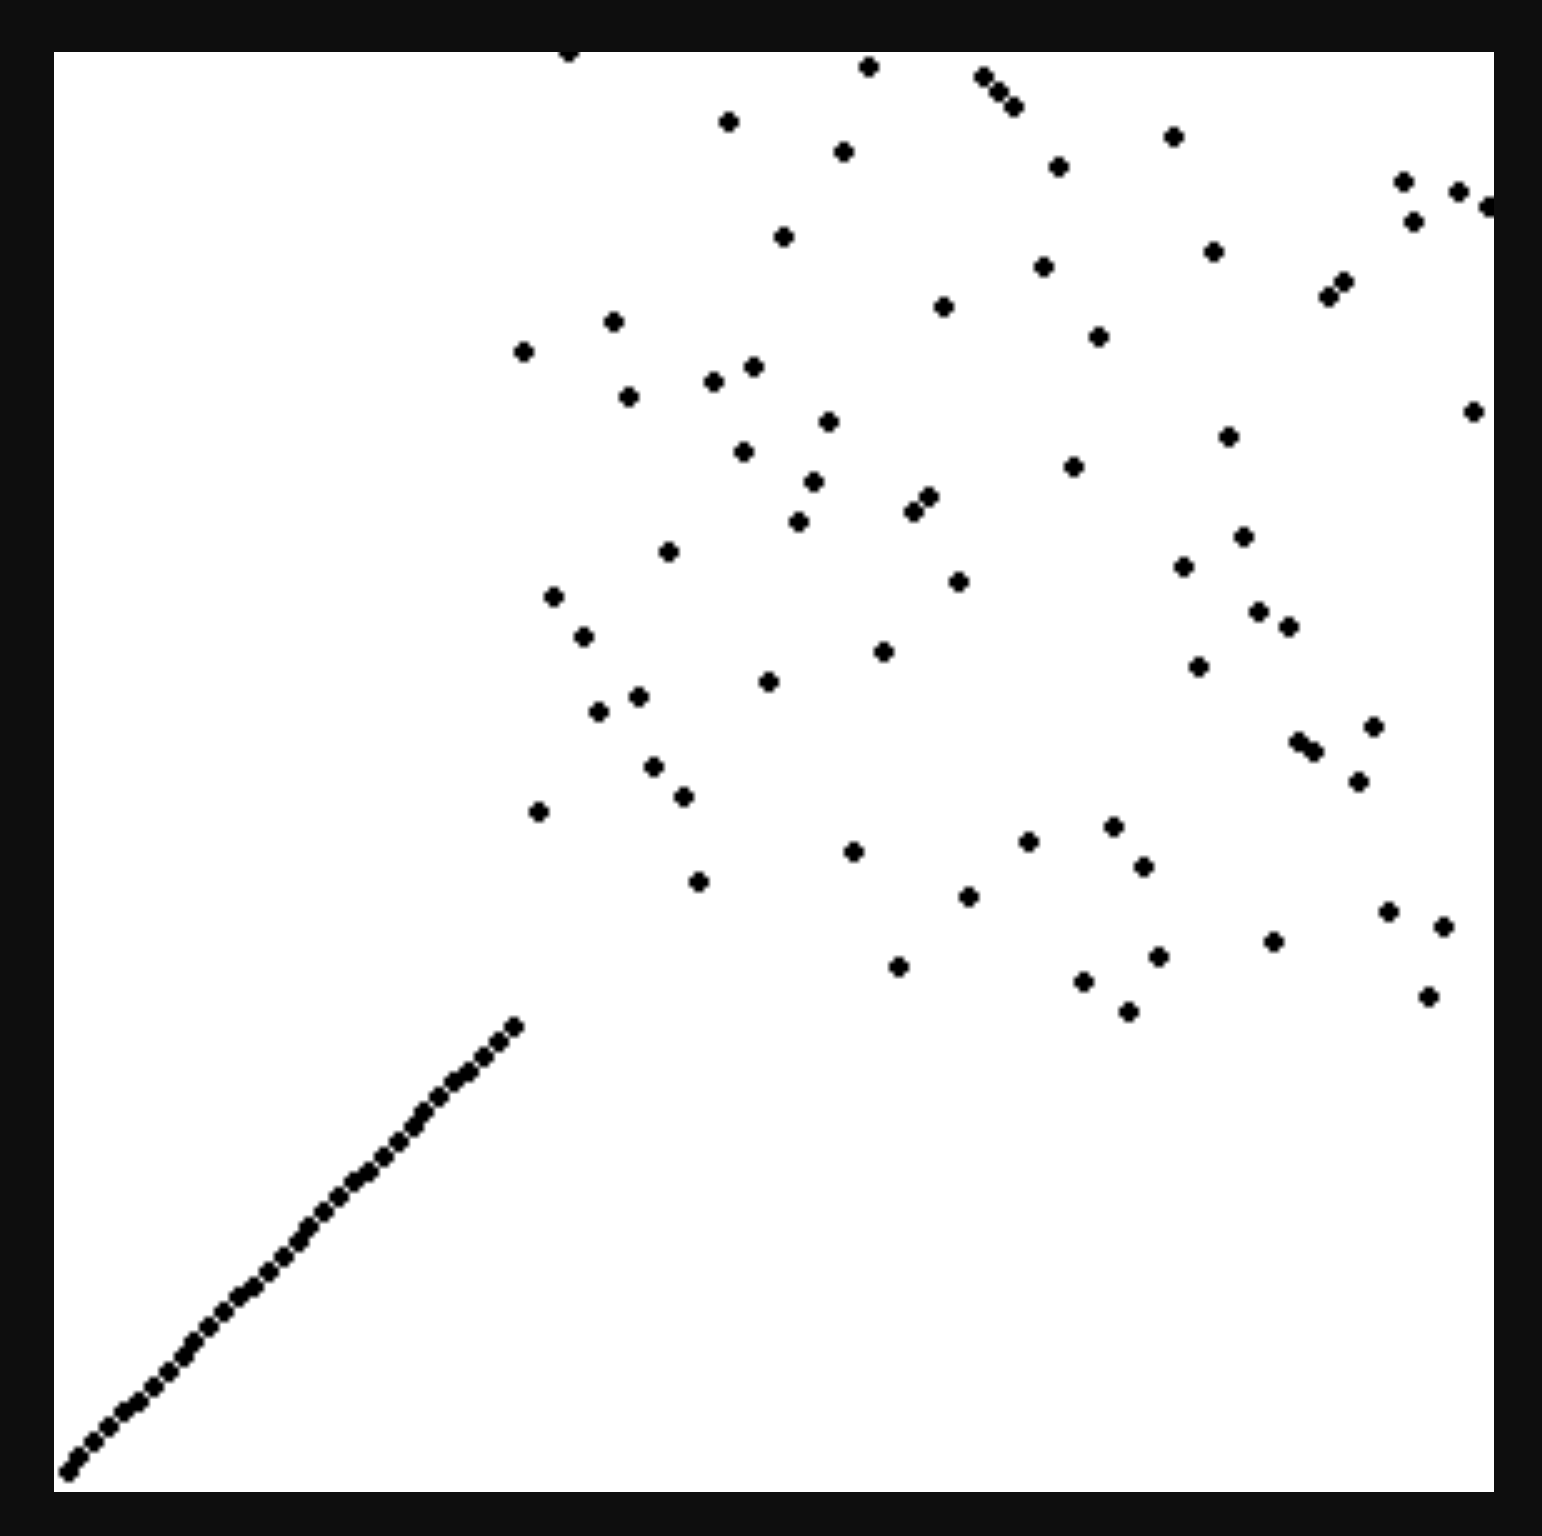
\includegraphics[width=\textwidth]{../images/ssort_gif.png}

  (\href{https://upload.wikimedia.org/wikipedia/commons/b/b0/Selection_sort_animation.gif}{animation})
\end{minipage}

\end{footnotesize}
\end{frame}

\end{document}
